% For submission and review of your manuscript please change the command to 
\documentclass[manuscript, screen]{acmart}
% When submitting camera ready or to TAPS, please change the command to 
% \documentclass[sigconf]{acmart}

\pagestyle{plain}

\usepackage{xspace}
\usepackage{siunitx}
\DeclareSIUnit{\fps}{fps}
\usepackage[inline]{enumitem}
\usepackage{multicol}
\usepackage{multirow}
\usepackage{graphicx} % Ensure graphicx is included for figures

\newcommand{\etal}{\emph{et~al.\xspace}}
\newcommand{\ie}{\emph{i.e.}, }
\newcommand{\eg}{\emph{e.g.}, }
\newcommand{\etc}{\emph{etc.\xspace}}
\newcommand{\vxv}[2]{$#1\!\times\!#2$}

\AtBeginDocument{%
  \providecommand\BibTeX{{%
    Bib\TeX}}}

% Rights management information. 
% \copyrightyear{2025}
% \acmYear{2025}
% \setcopyright{acmcopyright}
% \acmConference[TOMM '25]{ACM Transactions on Multimedia Computing, Communications, and Applications}{TBD 2025}{TBD}
% \acmBooktitle{ACM Transactions on Multimedia Computing, Communications, and Applications (TOMM '25)}
% \acmDOI{TBD}
% \acmISBN{TBD}

\begin{document}

\title[PointStream]{PointStream: A Hybrid Semantic Codec with Generative Reconstruction for Live Video Streaming}

\author{Emanuele Artioli}
\email{emanuele.artioli@aau.at}
\orcid{0009-0007-9921-0006}
\affiliation{
  \institution{Alpen-Adria-Universitaet}
  \city{Klagenfurt}
  \state{Kaernten}
  \country{Austria}
}
\author{Daniele Lorenzi}
\email{daniele.lorenzi@aau.at}
\orcid{0000-0003-3689-6315}
\affiliation{
  \institution{Alpen-Adria-Universitaet}
  \city{Klagenfurt}
  \state{Kaernten}
  \country{Austria}
}
\author{Farzad Tashtarian}
\email{farzad.tashtarian@aau.at}
\orcid{0000-0002-5584-6690}
\affiliation{
  \institution{Alpen-Adria-Universitaet}
  \city{Klagenfurt}
  \state{Kaernten}
  \country{Austria}
}
\author{Christian Timmerer}
\email{christian.timmerer@aau.at}
\orcid{0000-0002-0031-5243}
\affiliation{
  \institution{Alpen-Adria-Universitaet}
  \city{Klagenfurt}
  \state{Kaernten}
  \country{Austria}
}

\begin{abstract}
As video resolutions and frame rates continue to rise, a key challenge in video streaming is maintaining high quality under constrained bandwidth. While recent work explores semantic compression, many approaches still transmit large amounts of pixel data or are unsuitable for live applications. We introduce PointStream, a hybrid, object-centric streaming framework designed for real-time video. PointStream classifies scenes based on background motion: scenes with complex motion are encoded with a traditional codec like AV1, while stable scenes (those with static or simple motion) are processed by our neural codec. For these stable scenes, the background is modeled as a single panoramic image, and its motion is described by a stream of homography matrices. The server then transmits only high-level information about dynamic foreground objects—such as poses and minimal appearance descriptors. Full frames are reconstructed on the client by warping the background panorama and using generative models to synthesize the foreground. This approach is demonstrated on a variety of content, with a focus on sports videos. Experiments show that PointStream achieves adequate perceptual quality (e.g., 60 VMAF) at bitrates under 200 Kbps, whereas state-of-the-art live codecs require 7 to 10 times more bandwidth to reach the same quality. The modular implementation and dataset will be made available upon acceptance.
\end{abstract}

\renewcommand{\shortauthors}{Emanuele Artioli, et al.}

\begin{CCSXML}
<ccs2012>
    <concept>
        <concept_id>10010147.10010178.10010224.10010245.10010252</concept_id>
        <concept_desc>Computing methodologies~Object identification</concept_desc>
        <concept_significance>500</concept_significance>
        </concept>
    <concept>
        <concept_id>10010147.10010178</concept_id>
        <concept_desc>Computing methodologies~Artificial intelligence</concept_desc>
        <concept_significance>500</concept_significance>
        </concept>
    <concept>
        <concept_id>10002951.10003227.10003251.10003255</concept_id>
        <concept_desc>Information systems~Multimedia streaming</concept_desc>
        <concept_significance>500</concept_significance>
        </concept>
    <concept>
        <concept_id>10010147.10010371.10010395</concept_id>
        <concept_desc>Computing methodologies~Image compression</concept_desc>
        <concept_significance>500</concept_significance>
        </concept>
</ccs2012>
\end{CCSXML}

\ccsdesc[500]{Computing methodologies~Object identification}
\ccsdesc[500]{Computing methodologies~Artificial intelligence}
\ccsdesc[500]{Information systems~Multimedia streaming}
\ccsdesc[500]{Computing methodologies~Image compression}

\keywords{HTTP adaptive streaming, Generative AI, Semantic Video Coding, Quality of Experience}

\maketitle

\section{Introduction}
Modern video codecs consume excessive bandwidth by encoding important motion with the same priority as irrelevant visual details--an increasingly critical inefficiency, given that video streaming is ubiquitous and accounts for 65\% of global Internet traffic~\cite{sandvine}. While traditional codecs like High Efficiency Video Codec (HEVC or H.265)~\cite{h265_overview} or AOMedia Video~1 (AV1)~\cite{av1_overview}, \etc ~employ compression techniques such as motion estimation to significantly reduce redundancy, they still encode full frames and treat them as sequences of blocks. As a result, they lack higher-level semantic understanding, give equal priority to imperceptible background changes, and fail to exploit predictable object appearance and movement. The ongoing shift to 4K (\vxv{3840}{2160}) resolution and beyond makes these inefficiencies more pronounced.

In contrast, the human visual system processes scenes with remarkable efficiency. Rather than uniformly parsing the entire visual field, the brain focuses attention on salient objects and motion, using peripheral vision to gather low-resolution contextual cues~\cite{cajar2016spatial}. Moreover, the brain leverages prior visual experience to anticipate familiar patterns, allowing it to infer and reconstruct missing or occluded information based on learned expectations~\cite{serences2006selective}. This combination of object-centric processing and predictive inference yields a far more efficient representation of dynamic environments than conventional video compression methods achieve.

Inspired by this efficiency, we propose {\em PointStream}, a novel hybrid codec for live video streaming that prioritizes semantically meaningful content. PointStream's pipeline begins by classifying scenes based on background motion. Scenes with complex, unpredictable motion are gracefully handed off to a traditional codec like AV1, ensuring that the system is never worse off than the standard alternative, save for a minor analysis overhead. For scenes with static or simple motion (e.g., pans or zooms), our neural codec takes over. It identifies and isolates objects of interest, encoding their motion into a lightweight representation of keypoints derived from pose estimation models. The background is modeled separately, either as a single static image or as a larger stitched panorama with corresponding transformation matrices. The client receives this compact data packet and uses generative models to reconstruct high-fidelity video frames. This approach differs from foveated streaming, which saves bandwidth by degrading the quality of the visual periphery. While effective, foveated methods can lead to a poor experience if the viewer's focus shifts unexpectedly to a low-quality region. PointStream avoids this by always preserving a high-quality background, ensuring a perceptually stable experience while still achieving significant bandwidth savings.

The primary contributions of this work include:
\begin{itemize}[topsep=0pt,itemsep=0pt,leftmargin=*]
\item \textbf{A hybrid semantic video codec} that intelligently routes video segments to either a traditional codec or our neural codec based on scene complexity, optimizing for both quality and efficiency.
\item \textbf{An efficient server-side pipeline} that uses modern deep learning models for object detection (YOLOv12), pose estimation (MMPose), and background modeling to create a low-bitrate semantic representation.
\item \textbf{A modular end-to-end system} designed for research, allowing for pluggable components and detailed performance instrumentation to facilitate ablation studies.
\end{itemize}

\section{Related Work}

\subsection{Traditional video coding and streaming}
Leveraging the Hypertext Transfer Protocol (HTTP) as a ubiquitous and interoperable foundation, HTTP Adaptive Streaming (HAS) delivers video content over the Internet under varying network conditions. HAS enables clients to switch between video qualities based on real-time measurements of network throughput and buffer levels. Adaptive Bitrate (ABR) control, typically implemented on the client side, represents the dominant strategy for streaming at scale~\cite{sani2017abr}. Standardized HAS variants, such as Dynamic Adaptive Streaming over HTTP (DASH)~\cite{Stockhammer2011} and HTTP Live Streaming (HLS)~\cite{AppleHLS}, partition videos into small HTTP-delivered segments and encode them at multiple quality levels. Clients select the version of each upcoming segment that best matches predicted network conditions, reducing rebuffering and enhancing the overall quality of experience~\cite{QoEWhitePaper}.

As video resolutions and streaming demands continue to rise, more advanced codecs emerge to improve compression efficiency. State-of-the-art standards such as Versatile Video Coding (VVC or H.266)~\cite{vvc_overview} and AV1~\cite{av1_overview} reduce bitrates by up to 50\% compared to their predecessors, HEVC and VP9~\cite{vp9_overview}, while maintaining similar visual quality. However, these gains come at the cost of significantly increased computational complexity, particularly during encoding, which limits their practicality for real-time or low-power applications. This trade-off prompts ongoing exploration of alternative compression techniques.

\subsection{Beyond traditional codecs}
Artificial intelligence (AI) techniques offer potential advancements in video streaming. AI-driven approaches enhance traditional codec pipelines by integrating AI modules that optimize specific components, such as rate control, motion estimation, or bitrate allocation, without altering the overall codec architecture~\cite{liu2020deep, lu2019dvc}. These hybrid methods improve compression efficiency and visual quality while remaining compatible with existing standards. In contrast, end-to-end neural video codecs replace the entire traditional pipeline with deep learning models that directly learn compact representations of video content from data~\cite{lu2019dvc, chen2021nerv}. While these fully learned systems match or even exceed the compression rates of conventional codecs, they introduce even higher computational complexity, particularly during encoding, which limits their practicality for real-time or resource-constrained scenarios.

As the computational complexity of modern video codecs continues to grow, especially on the encoding side, researchers explore ways to shift some of the processing load to the client. This shift leads to the development of techniques that enhance video quality after transmission, leveraging the increasing capabilities of consumer hardware. Notable examples include client-side frame interpolation~\cite{niklaus2020softmax, xu2019quadratic} and super-resolution~\cite{ledig2017photo}, which improve perceived visual quality independently of network conditions. These approaches represent a promising direction in research, optimize natively for the rapidly increasing capabilities of modern Graphics Processing Units (GPUs), and offer a practical way to improve quality without increasing bandwidth. However, they typically operate at the pixel or texture level, applying enhancements uniformly across the frame without considering semantic content or viewer attention, limiting their potential efficiency.

\subsection{Semantic video streaming}
Research in semantic video streaming addresses these limitations by analyzing and understanding high-level scene semantics to improve encoding efficiency. Instead of treating all pixels as equally important, semantic systems prioritize key foreground objects for detailed encoding. Techniques for object detection and tracking, such as Mask R-CNN~\cite{he2017mask} or transformer-based object trackers~\cite{meinhardt2022trackformer}, enable the isolation of moving elements. 
A particularly relevant approach is **foveated streaming**, inspired by the human eye's fovea, which perceives the center of the visual field in high resolution and the periphery in low resolution. Foveated systems save bandwidth by encoding the periphery of a video frame at a lower quality than the center, often tracking the viewer's gaze to dynamically update the high-quality region~\cite{foveated_streaming}. While effective, this approach can degrade the user experience if the gaze prediction is inaccurate or if salient events occur in the low-quality periphery. PointStream offers an alternative by maintaining a consistently high-quality background, focusing its compression efforts on the representation of moving foreground objects, thereby decoupling bandwidth savings from peripheral quality degradation.
Another approach is the use of skeletal models for human representation also gain traction, especially in applications like telepresence and low-bandwidth activity capture. Methods like OpenPose~\cite{cao2017realtime} and BlazePose~\cite{bazarevsky2020blazepose} generate lightweight yet expressive skeletal representations of motion, which streaming systems transmit in place of full pixel data. The client reanimates or renders these representations, significantly reducing bandwidth without compromising perceived quality or interactivity. Integrating such semantic abstractions into streaming pipelines marks a critical shift toward perceptually optimized video delivery.

Despite its potential, semantic streaming remains primarily explored in adjacent domains rather than in core video compression tasks, \eg video conferencing~\cite{zhang2020semantic3d, liu2023semconf}, 360-degree video streaming~\cite{qian2018flare, xu2020seaware}, and autonomous driving~\cite{wang2021longshortnet}. 
Only a few studies focus on applying semantic understanding to enhance video compression directly~\cite{zhu2019semanticadaptive, hu2020taskoriented}. These approaches show promise, but they often stop at detection or segmentation and lack optimized methods for encoding and regenerating the detected objects, limiting their ability to fully exploit the bandwidth savings achievable with semantically driven compression.

\begin{figure*}
    \centering
    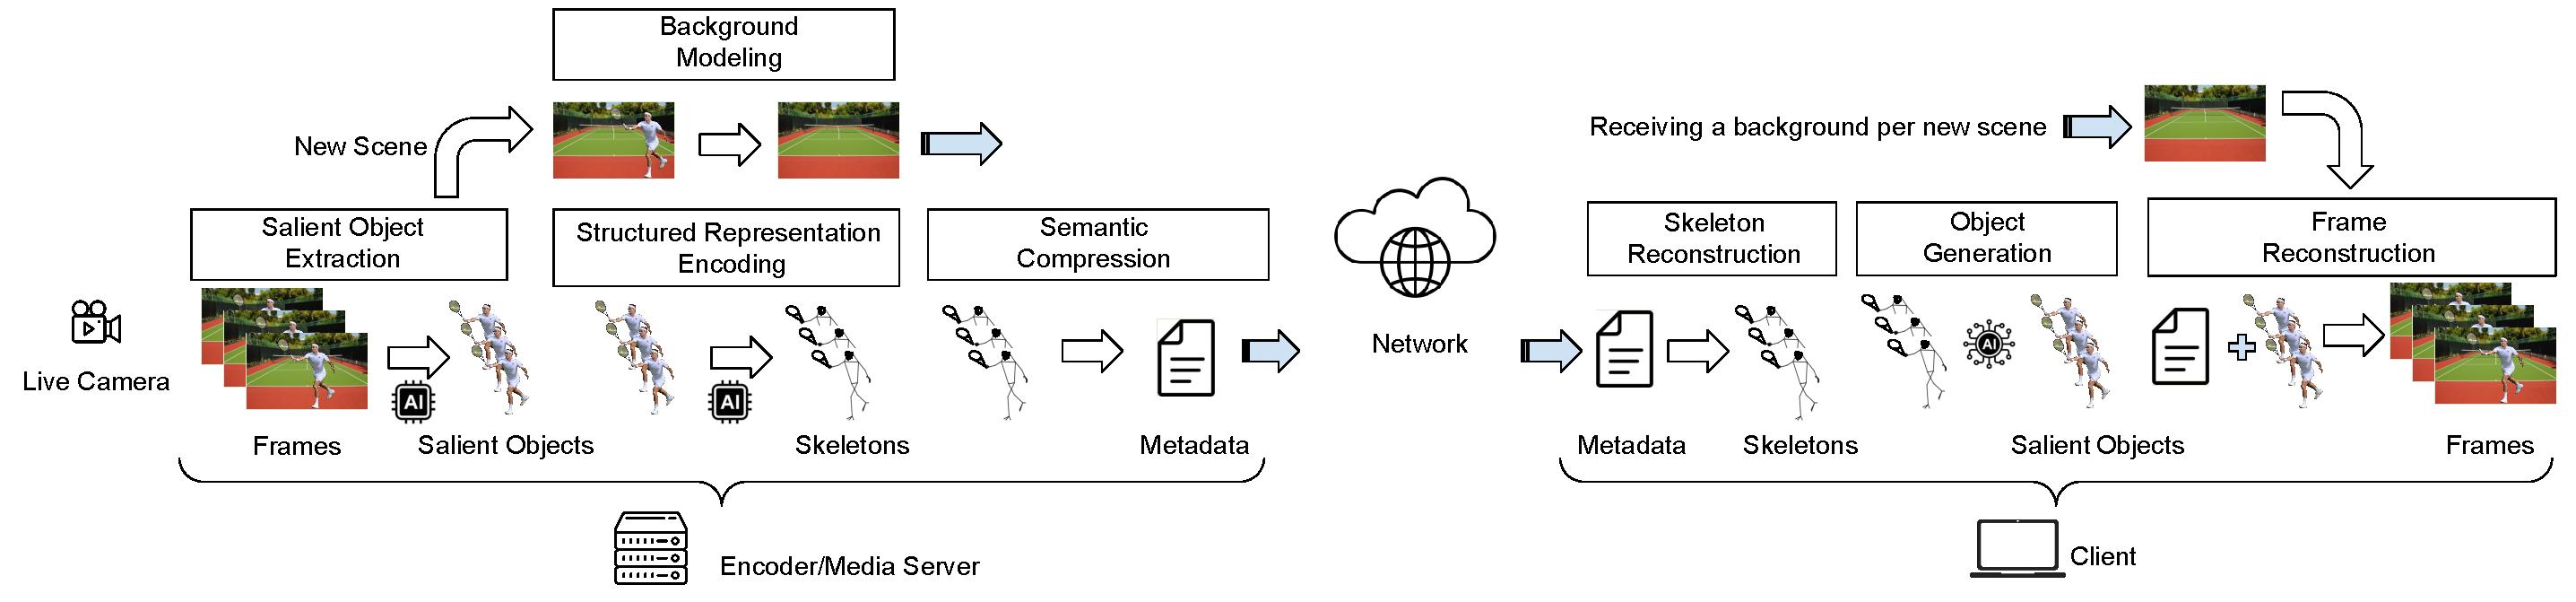
\includegraphics[width=1\linewidth]{figures/PS-overview.pdf}
    \caption{Conceptual overview of PointStream integration into the video streaming pipeline.}
    \label{fig:ps-overview}
\end{figure*}

\subsection{GenAI-based video streaming}
Advances in Generative AI (GenAI) enable impressive progress in image and video synthesis, with models that produce photorealistic scenes and animate static content~\cite{ramesh2021dalle, ho2020ddpm, isola2017pix2pix}. These models learn high-level semantic representations of objects and their motion, which makes them well-suited for applications in video streaming---particularly for reconstructing visual information from compact, abstract encodings. Despite this potential, most generative approaches remain decoupled from real-time streaming pipelines. They typically rely on private datasets and require significant computational resources to train and deploy. As a result, developers mainly use them for offline generation or post-processing, rather than integrating them directly into video compression systems.

Recent attempts explore the possibilities of integrating generative models into video streaming pipelines. For example, ELVIS~\cite{elvis} proposes a client-side inpainting framework that removes low-importance regions from transmitted frames and fills them in using a generative model at the client. This reduces the amount of background elements transmitted over the network. Although innovative, this solution still relies on traditional block-based compression and lacks deeper integration of semantic segmentation and reconstruction. As a result, it does not fully exploit object-level priors or motion-aware representations and treats each block as an isolated unit, rather than as part of a coherent object or action.

While previous work advances compression efficiency, semantic analysis, and generative reconstruction in isolation, these developments largely evolve along parallel tracks. Traditional codecs focus on low-level signal optimization, semantic systems stop at detection without optimized encoding, and generative models remain underutilized within streaming pipelines. The intersection of these trajectories reveals a clear opportunity: a unified framework that combines semantic understanding, compact representation, and generative reconstruction to enable efficient, high-quality video streaming. PointStream emerges in this space, introducing a fully object-based encoding approach that leverages scene semantics to minimize redundancy and uses generative models to reconstruct video content intelligently on the client side.


\section{Problem Description and Motivation}
To evaluate whether our approach brings meaningful improvements, we first establish a baseline by measuring the performance of current state-of-the-art codecs under constrained bandwidth conditions, using a tennis match segment at 4K resolution, a framerate of \SI{50}{\fps}, and \SI{8}{\second} of duration as our test case.
As our reference codec, we select HEVC due to its widespread adoption and high compression efficiency. 
We encode the target video\footnote{\url{https://www.youtube.com/watch?v=7QoKrvOvIGw&t=88s}, last access: 2025-09-18.} at each bitrate among the representations in the Apple HLS bitrate ladder~\cite{AppleHLS}, which results in qualities ranging from \SI{27}{VMAF} at 360p (\vxv{640}{360}) and 145\,Kbps, up to nearly flawless reconstruction at 4K and 11\,Mbps. 

Given the structured nature of many video types, particularly sports, we explore a content-aware alternative that exploits the inherent redundancy in the scene. 
A typical broadcast consists of 
\begin{enumerate*}[label=\textit{(\roman*)}] 
\item a static or predictably moving background (court, audience), and 
\item a few dynamic elements (players, rackets, ball)
\end{enumerate*}.
Instead of encoding all pixels in every frame, we propose a simple yet effective optimization:
\begin{itemize}[topsep=0pt,itemsep=0pt,leftmargin=*]
    \item Extract and store only the moving objects as separate video streams.
    \item Compress and store the background as a single static image.
\end{itemize}
This approach ignores irrelevant motion (\eg minor spectator movements), while significantly reducing bitrate consumption. For our test video, this method reduces the data size by approximately \qty{60}{\percent} compared to the standard 4K HEVC encoding.

Despite these impressive gains, this method still requires encoding full pixel-based representations of moving objects. We observe that players are humans whose motion can be efficiently represented using structured pose information. 
Leveraging this insight, we take an additional step:
\begin{itemize}[topsep=0pt,itemsep=0pt,leftmargin=*]
\item Instead of encoding pixel-level video streams, we extract 2D pose trajectories using a state-of-the-art pose estimator and represent motion as a sequence of keypoints.
\item We employ a lightweight generative model (a cGAN~\cite{isola2017pix2pix}) to reconstruct plausible visual representations of the players conditioned on these pose sequences.
\end{itemize}
This transformation yields another substantial reduction in data size, from the previous \SI{950}{KB} and \SI{1.2}{MB} to \SI{230}{KB} and \SI{294}{MB}, or about \qty{75}{\percent} smaller than the object-video approach, and a total reduction from \SI{4.55}{MB} to \SI{2.92}{MB}, another \qty{36}{\percent} size drop.
% Once more, we forgo to calculate VMAF for these experiments, and instead assume that the client side generative model would be able to replicate players without noticeable artifacts.

We note that these results assume that the perceptual impact of certain approximations is negligible. 
In particular, encoding the background as a static image may reduce objective quality metrics such as VMAF, but we posit that this does not reflect a meaningful drop in perceived quality, given the minimal motion and low saliency of those background elements.
Similarly, in the pose-based reconstruction case, we assume that the generative model produces visually plausible outputs sufficient to maintain perceived fidelity. 
While these assumptions simplify the evaluation, they are reasonable within the controlled scope of this illustrative example.

Although not intended as a rigorous or statistically comprehensive evaluation, this stepwise transformation, from full-frame encoding, to object-background separation, to structured motion-based representation, highlights the potential of a content-aware, human-centric approach. 
These insights directly inform the design of our proposed system, \emph{PointStream}, which generalizes this paradigm into a scalable and modular semantic live streaming pipeline.


\section{System Design}
PointStream is built around a layered representation of a video chunk rather than a monolithic encoded frame sequence. The central design decision is to separate what must be remembered from what can be recomputed. Static structure is summarized as a background panorama, foreground motion is expressed as sparse semantic events, and any remaining pixel detail is preserved in a residual stream. This makes the system hybrid in a deeper sense than a simple codec switch: semantics carry the scene structure, while conventional coding remains the safety net that preserves fidelity where the semantic layer is incomplete.

The payload contract in \texttt{src/shared/schemas.py} makes this separation explicit. A \texttt{VideoChunk} defines the time span and geometry of the source. A \texttt{PanoramaPacket} stores the camera-grounded background, including selected frame indices, camera poses, and homography matrices. \texttt{ActorPacket} objects carry sparse keyframe events, optional mask frames, and appearance descriptors for humans. \texttt{RigidObjectPacket} and \texttt{BallPacket} provide a path for non-human motion, which is important because the design is not tied to a single object class. Finally, a \texttt{ResidualPacket} preserves the conventional video stream for information not explained by the semantic representation. In aggregate, these packets form a compositional scene description rather than a collection of unrelated side channels.

\subsection{Semantic encoding pipeline}

To build this layered representation, PointStream employs a staged encoder pipeline that progressively annotates the scene with increasing semantic richness. The pipeline performs the following sequence of operations on each frame:

\subsubsection{Object Detection}
The first stage identifies and tracks foreground objects. Two detector backends are available, reflecting a tradeoff between fixed and open-vocabulary detection:
\begin{itemize}[topsep=0pt,itemsep=0pt,leftmargin=*]
    \item \textbf{YOLOv8 Nano (YOLO26)} uses a traditional fixed-class detector trained on COCO, identifying persons and tennis rackets. This backend is computationally efficient and requires no external configuration beyond the base model.
    \item \textbf{YOLOE (Open-vocabulary variant)} extends YOLOv8 with a text encoder (MobileCLIP) to enable open-vocabulary detection based on caption prompts. This allows detection customization per deployment, \eg ``tennis player'' or ``badminton player'', without retraining. The text encoder weights are cached locally to ensure deterministic inference.
\end{itemize}
Both detectors include frame-level tracking to maintain consistent identity across time. When tracking loss occurs (e.g., during occlusion), a recovery heuristic searches the region around the last known position to re-establish the track. The pipeline enforces a minimum of two players and two rackets per frame; if the detector misses objects, they are reconstructed by temporal interpolation or simple positional priors to ensure consistent semantic structure.

\subsubsection{Pose Estimation}
Once objects are identified, human actors are further annotated with skeletal motion via pose estimation. Two pose backends are available:
\begin{itemize}[topsep=0pt,itemsep=0pt,leftmargin=*]
    \item \textbf{YOLO Pose (YOLOv8 Pose)} uses the built-in pose head of YOLOv8, producing COCO-17 keypoint coordinates (17 joints with confidence values). The output is converted to DWPose/OpenPose-18 format by synthesizing the neck joint from shoulder positions when both are above a confidence threshold (0.2).
    \item \textbf{DWPose (TorchScript)} runs a standalone OpenPose-compatible detector optimized for sports contexts. This backend processes each actor crop and directly outputs the 18-joint representation. It is typically more robust to occlusion and unusual poses than YOLO Pose but at higher computational cost.
\end{itemize}
Both backends extract the actor crop with 10\% padding around the bounding box to provide context, then apply the pose model to infer keypoint locations. Pose keypoints are stored as $(x, y, \text{confidence})$ triplets and serve as the primary semantic representation of motion in the ActorPacket. Keyframes are emitted when the Euclidean distance of flattened pose coordinates exceeds a configurable threshold (default 20.0 pixels), implementing an adaptive motion-driven rate control that sends fewer keyframes during slow play and more during rapid movement.

\subsubsection{Instance Segmentation}
To provide spatial guidance and optional mask-based compositing, the pipeline optionally performs instance segmentation. Three backends are available, representing different quality-speed tradeoffs:
\begin{itemize}[topsep=0pt,itemsep=0pt,leftmargin=*]
    \item \textbf{No-op segmentation} skips masking entirely. This is the lowest-bandwidth option and is useful when mask-guided compositing is disabled or when segmentation latency is prohibitive.
    \item \textbf{YOLO Segmentation (YOLOv8-Seg)} applies the segmentation head of YOLOv8 to each actor crop, producing a binary mask. The implementation extracts polygon coordinates when available for more compact representation. This is fast and well-integrated with the detection backend.
    \item \textbf{YOLOE Segmentation} provides open-vocabulary segmentation using the same caption-based prompting as open-vocabulary detection, enabling customized mask targets per deployment.
    \item \textbf{SAM (Segment Anything Model)} uses the Segment Anything Model (SAM3 or SAM) with bounding-box prompts, providing higher-quality segmentation at increased computational cost. SAM operates on the full frame rather than crops, accepting the actor bounding box as a prompt and producing high-fidelity instance masks.
\end{itemize}
Masks are stored in the ActorPacket using a configurable codec (RLE, bitpacking, PNG, or polygon) to balance bandwidth and reconstruction fidelity.

\subsubsection{Background Modeling}
Parallel to foreground annotation, the background is modeled as a reusable geometric structure via the BackgroundModeler. This component:
\begin{itemize}[topsep=0pt,itemsep=0pt,leftmargin=*]
    \item Estimates optical flow using the KLT (Kanade-Lucas-Tomasi) algorithm to track frame-to-frame motion.
    \item Selects keyframes based on cumulative translation thresholds (default 30 pixels) to identify frames where substantial new background content enters the view.
    \item Constructs a panorama by stitching selected keyframes via median fusion and homography warping, creating a larger canvas that encompasses most scene content.
    \item Computes per-frame homography matrices that describe how to warp the panorama into the current camera viewpoint, effectively converting camera motion from the pixel domain to the geometric transform domain.
\end{itemize}
The PanoramaPacket stores the stitched panorama image (in PNG or JPEG format), the homography matrices for all frames, and metadata about which frames were used for stitching. On the client, these homographies are applied via perspective warping to reconstruct the background for each frame, achieving high-quality geometry with minimal transmitted pixels.

\subsubsection{Ball and Rigid Object Tracking}
For scenes where non-human motion is salient (e.g., ball tracking in tennis), the pipeline includes specialized detectors:
\begin{itemize}[topsep=0pt,itemsep=0pt,leftmargin=*]
    \item \textbf{Ball Extraction} uses background subtraction and blob detection, computing per-frame differences between the original and warped background, then identifying connected components above a minimum area threshold (default 6 pixels). The detector adapts to motion by interpolating trajectory continuity across frames.
    \item \textbf{Rigid Object Detection} provides a slot for additional tracked objects using trajectory-based representation, stored in RigidObjectPacket with similar keyframe-based event encoding as human actors.
\end{itemize}
Both are optional and can be disabled for faster encoding when the application does not require sub-object tracking.

\subsubsection{Reference Extraction and Residual Encoding}
Finally, the encoder materializes compact visual references and residual fallback:
\begin{itemize}[topsep=0pt,itemsep=0pt,leftmargin=*]
    \item \textbf{Actor References} extracts a single JPEG crop per tracked actor from the first confident detection. Crops include configurable padding (default 10\%) and JPEG quality (default 75) to balance appearance fidelity and bandwidth. These references are transmitted in the SceneActorReference structure and provide visual identity cues for appearance synthesis on the client.
    \item \textbf{Residual Stream} encodes pixel differences between the full frame and the composite of warped background plus actor masks, weighted by an importance map. Two importance strategies are available: binary (1.0 where actors present, 0.0 elsewhere) or uniform. The residual is encoded with FFmpeg and transmitted as a fallback video stream.
\end{itemize}

\subsection{Background as geometric state}
The most distinctive part of the design is the treatment of the background as a reusable geometric state. Instead of retransmitting full frames whenever the camera moves, PointStream represents the background as a panorama that can be reprojected into the current view with homography matrices. In other words, camera motion is moved from the pixel domain into the transform domain. This is a strong compression lever because many broadcast scenes contain a mostly stable canvas with a changing viewpoint, but relatively little new background information from frame to frame.

This design also explains why the background packet stores both a panorama image and a homography sequence. The panorama provides the visual substrate, while the per-frame transforms encode the motion needed to recover the live viewpoint. The client therefore does not merely decode a background image; it reconstructs the current camera view by warping a stable reference layer. The result is a background that remains high-quality even when foreground content is highly dynamic.

\subsection{Sparse foreground semantics}
Foreground objects are represented sparsely and semantically rather than as dense video. Human actors are encoded through pose-oriented events that are only emitted when the pose changes enough to justify a new keyframe. This is a deliberate rate-control strategy: the number of transmitted events depends on motion complexity, not on the frame rate of the source. Optional mask frames and appearance references extend the representation when the client needs stronger spatial guidance, but they do not change the core abstraction. The pose delta threshold is the primary tuning knob for bandwidth: higher thresholds reduce event density but may miss rapid movements, while lower thresholds preserve finer motion at increased bitrate.

The same pattern extends to rigid objects and balls. These packets are included because real scenes are not only about people, and a robust semantic codec should be able to carry non-human motion without redesigning the transport layer. This is also where the current implementation shows its longer-term potential: the system already has separate slots for human pose, object trajectories, and residual pixels, so additional object classes can be added without changing the fundamental architecture.

\subsection{Reconstruction as synthesis plus compositing}
On the client, PointStream reconstructs frames by combining three sources of information: warped background geometry, sparse object semantics, and a residual stream. The important design point is that reconstruction is not a single generator call. It is a staged process that first densifies sparse motion, then recovers object appearance, and finally composites the result back into the transmitted background. This makes the system easier to adapt because the appearance model, the compositor, and the geometric background model are all independently replaceable.

Generative AI is therefore best understood as an optional reconstruction strategy inside a larger scene model, not as the core abstraction of the codec. When a heavy generative backend is available, the client can synthesize richer foreground appearance. When it is not, the rest of the pipeline still works because the structural contract is already there. That separation is what gives the design practical value: the system can exploit modern generative models without becoming dependent on them.

\section{Implementation}
The current codebase realizes this design in \texttt{src/main.py} as a single-chunk pipeline with a small CLI front end. The top-level runner parses the experiment configuration, applies environment overrides, resolves the source video, and then executes one encode transport decode cycle. If no input is supplied, the code generates a synthetic tennis-like clip so the entire stack remains runnable without external assets. That fallback is not just a convenience feature; it makes the system testable and reproducible in the absence of a full dataset.

\subsection{Encoder Pipeline Assembly}
The encoder itself is implemented by \texttt{EncoderPipeline} in \texttt{src/encoder/orchestrator.py}. Internally, it is organized as a DAG using \texttt{DAGOrchestrator}, which is the right abstraction for this kind of system because the semantic payload has real dependencies: actor extraction must precede pose export, the panorama depends on frame states, actor references depend on those same states, and the residual is built last from the assembled semantic payload. The graph contains explicit nodes for the chunk, actor bundle, actors, frame states, panorama, actor references, rigid objects, ball, and residual. That structure makes the execution order clear and also leaves room for parallel scheduling when a tagged execution pool is enabled.

\subsubsection{Actor Extraction}
The \texttt{ActorExtractor} class in \texttt{src/encoder/actor\_components.py} implements the full pipeline described in Section~\ref{sec:encoding}. It accepts configurable parameters for each stage:
\begin{itemize}[topsep=0pt,itemsep=0pt,leftmargin=*]
    \item \textbf{Detector backend:} \texttt{--detector} with options \texttt{yolo26} or \texttt{yoloe}. YOLO26 uses YOLOv8 Nano; YOLOE uses MobileCLIP-augmented open-vocabulary detection.
    \item \textbf{Detector caption:} \texttt{--detector-caption} for YOLOE customization (default: ``tennis player'').
    \item \textbf{Pose estimator:} \texttt{--pose-estimator} with options \texttt{yolo} or \texttt{dwpose}. Both produce 18-joint DWPose format.
    \item \textbf{Segmenter backend:} \texttt{--segmenter} with options \texttt{yolo}, \texttt{yoloe}, \texttt{sam3}, \texttt{sam}, or \texttt{none}. Each produces a binary mask in configurable codec.
    \item \textbf{Segmenter caption:} \texttt{--segmenter-caption} for open-vocabulary segmenters.
    \item \textbf{Pose delta threshold:} \texttt{--payload-pose-delta-threshold} (default 20.0 pixels) controls keyframe emission rate.
    \item \textbf{Debug keyframes:} \texttt{--disable-debug-keyframes} to skip skeletal visualization.
    \item \textbf{Mask metadata inclusion:} Controlled by \texttt{--compositing-mask-mode} (default \texttt{postgen-seg-client}).
    \item \textbf{Mask codec:} \texttt{--metadata-mask-codec} with options \texttt{auto}, \texttt{rle-v1}, \texttt{bitpack-z1}, \texttt{png}, \texttt{segmenter-native}, or \texttt{yolo-native}.
\end{itemize}
Internally, \texttt{ActorExtractor} runs detector, pose estimator, and segmenter in sequence on each frame, then applies a \texttt{PayloadEncoder} to convert frame states into sparse ActorPackets by tracking pose deltas and emitting keyframe events. Actors are associated with the detector output through spatial overlap, and rackets are linked to players via bounding-box proximity.

\subsubsection{Background Modeling}
The \texttt{BackgroundModeler} in \texttt{src/encoder/background\_modeler.py} constructs the panorama and homography matrices. It accepts raw frame states and optionally a pre-decoded video tensor for faster processing. Internally, it uses KLT-based optical flow tracking to identify keyframe candidates, selects frames based on cumulative translation (default 30 pixels), and stitches them into a panorama using median fusion and perspective warping. The output PanoramaPacket includes the stitched image in configurable format (PNG, JPEG), per-frame homography matrices, and metadata about selected frame indices.

\subsubsection{Ball and Rigid Object Detection}
The \texttt{BallExtractor} in \texttt{src/encoder/ball\_extractor.py} uses background subtraction with parameters:
\begin{itemize}[topsep=0pt,itemsep=0pt,leftmargin=*]
    \item \textbf{Difference threshold:} \texttt{--ball-difference-threshold} (default 18.0) for frame differencing.
    \item \textbf{Minimum blob area:} \texttt{--ball-min-blob-area} (default 6 pixels).
    \item \textbf{Detection frame size:} \texttt{--ball-max-side} (default 0, no downsampling) for optional resolution reduction.
\end{itemize}
The \texttt{ObjectTracker} in \texttt{src/encoder/mock\_extractors.py} provides a placeholder for rigid object trajectories. Both produce event-based packets with trajectory specifications.

\subsubsection{Reference Extraction}
The \texttt{ReferenceExtractor} in \texttt{src/encoder/reference\_extractor.py} extracts cropped JPEG images of each actor for use in appearance synthesis. Parameters:
\begin{itemize}[topsep=0pt,itemsep=0pt,leftmargin=*]
    \item \textbf{JPEG quality:} \texttt{--reference-jpeg-quality} (default 75).
    \item \textbf{Padding ratio:} \texttt{--reference-padding-ratio} (default 0.10 or 10\%).
\end{itemize}

\subsubsection{Residual Encoding}
The \texttt{ResidualCalculator} in \texttt{src/encoder/residual\_calculator.py} computes and encodes a residual stream. The importance map can be selected via \texttt{--importance-mapper} with options \texttt{binary} (1.0 where actors present, 0.0 elsewhere) or \texttt{uniform}. The residual is encoded using FFmpeg with the H.265/HEVC codec at a fixed quality level.

\subsection{Execution Pool and Parallelization}
By default (\texttt{--execution-pool inline}), the DAG runs synchronously. The alternative \texttt{--execution-pool tagged} activates \texttt{TaggedMultiprocessPool}, which distributes work across CPU and GPU processes based on function tags. The pool is configured with \texttt{--cpu-workers} and \texttt{--gpu-workers} (both default 1), allowing independent tuning of CPU-bound work (detection, pose estimation, background modeling) and GPU-bound work (residual synthesis). This architecture enables efficient utilization of multi-GPU systems or CPU farms.

\subsection{Serialization and Transport}
Once encoded, the payload is written through \texttt{DiskTransport} in \texttt{src/transport/disk.py}. The transport layer materializes the semantic packet into a chunk directory containing:
\begin{itemize}[topsep=0pt,itemsep=0pt,leftmargin=*]
    \item \texttt{metadata.msgpack}: Serialized EncodedChunkPayload with path references to external artifacts.
    \item \texttt{residual.mp4}: Encoded residual stream video.
    \item \texttt{panorama.png} (or \texttt{.jpg}): Stitched background image in selected format.
    \item \texttt{actor\_references/track\_*.jpg}: JPEG crops of each actor.
\end{itemize}
The transport layer also includes a \texttt{panorama\_encoder} selector (CLI option passed at transport creation) to choose panorama compression, supporting PNG and JPEG. This separation of artifacts into sidecar files makes the payload inspectable and testable without special infrastructure.

\subsection{Synthesis Engine and Client Reconstruction}
The \texttt{SynthesisEngine} in \texttt{src/shared/synthesis\_engine.py} is a shared utility used by both encoder (for residual computation) and decoder. It implements:
\begin{itemize}[topsep=0pt,itemsep=0pt,leftmargin=*]
    \item \textbf{Panorama warping:} Uses Kornia's perspective warp with batch processing to apply homography matrices to the panorama, reconstructing the background for each frame at the correct camera viewpoint.
    \item \textbf{Pose densification:} Unrolls sparse KeyframeEvent and InterpolateCommandEvent sequences into dense $(T, 18, 3)$ pose tensors via linear interpolation between keyframes.
    \item \textbf{Pose visualization:} Renders DWPose keypoints and skeletons onto a canvas for visualization or mask-based compositing.
\end{itemize}
The engine accepts configuration via environment variables: \texttt{POINTSTREAM\_GPU\_DTYPE} (default fp16 on CUDA) for compute precision, and \texttt{POINTSTREAM\_PANORAMA\_WARP\_BATCH\_SIZE} (default 4) for memory efficiency.

The \texttt{DecoderRenderer} in \texttt{src/decoder/mock\_renderer.py} orchestrates client-side reconstruction. It:
\begin{enumerate*}[label=\textit{(\roman*)}]
    \item Decodes reference crops from JPEG or in-memory bytes.
    \item Unrolls sparse actor poses into dense trajectories.
    \item Calls the synthesis engine to reconstruct background via warping and synthesize predicted foreground frames.
    \item Optionally applies GenAI appearance synthesis.
    \item Composites with residual stream via the ResidualCompositor.
\end{enumerate*}

\subsection{Generative AI Backends}
The GenAI path is controlled by environment variables. The system implements two main strategies via \texttt{src/decoder/genai\_compositor.py}:
\begin{itemize}[topsep=0pt,itemsep=0pt,leftmargin=*]
    \item \textbf{ControlNet baseline:} \texttt{--genai-backend controlnet} (default when enabled) uses Stable Diffusion v1.5 with OpenPose ControlNet. Accepts \texttt{--animate-anyone-window} (temporal context window, default 8 frames) and mask compositing modes.
    \item \textbf{AnimateAnyone:} \texttt{--genai-backend animate-anyone} uses the Moore-AnimateAnyone architecture for appearance-driven motion synthesis. Requires \texttt{--animate-anyone-repo-dir} pointing to the AnimateAnyone repository and \texttt{--animate-anyone-model-variant} (e.g., ``original'', ``finetuned\_tennis''). Additional options include \texttt{--animate-anyone-window} (temporal window), \texttt{--genai-preroll-frames} (frames to delay GenAI until residual stabilizes), \texttt{--animate-anyone-transparent-threshold} (alpha threshold for black-background masking), \texttt{--animate-anyone-adaptive-threshold} (enable adaptive border masking), and \texttt{--animate-anyone-alpha-smoothing} (temporal smoothing factor for alpha masks).
\end{itemize}
A lightweight \texttt{MockCompositor} is available for testing and always produces the synthesis output without generative synthesis. The compositing mode (\texttt{--compositing-mask-mode}) can be \texttt{alpha-heuristic} (rough alpha extraction), \texttt{metadata-source-mask} (use transmitted masks), or \texttt{postgen-seg-client} (segment generated frames on client using \texttt{--postgen-segmenter-backend}: \texttt{yolo} or \texttt{heuristic}).

\subsection{Runtime Configuration and Observability}
The CLI in \texttt{src/main.py} exposes all tunable parameters through argument parsing with validation. Running with \texttt{--help} shows all options. Key command groups:
\begin{itemize}[topsep=0pt,itemsep=0pt,leftmargin=*]
    \item \textbf{Video input:} \texttt{--input} (path or auto-generated), \texttt{--num-frames} (frame limit).
    \item \textbf{Execution:} \texttt{--execution-pool}, \texttt{--cpu-workers}, \texttt{--gpu-workers}.
    \item \textbf{Encoder components:} All actor extractor, ball extractor, reference, and residual options listed above.
    \item \textbf{GenAI:} \texttt{--enable-genai}, \texttt{--disable-genai}, \texttt{--genai-backend}, \texttt{--animate-anyone-*} family.
    \item \textbf{Debugging:} \texttt{--no-summary-file} (suppress output), \texttt{--disable-debug-keyframes}.
\end{itemize}
Runtime output is captured in a JSON summary that logs payload sizes and compression ratios, making ablation studies straightforward: changing a single option (e.g., segmenter backend or GenAI strategy) and re-running automatically reports the bandwidth and quality impact.

For development, the code emits debug artifacts (skeleton visualizations, flow maps, mask renderings) into a debug directory when \texttt{POINTSTREAM\_DEBUG\_ARTIFACT\_DIR} is set. The pipeline also restores working directory and environment variables after each run, ensuring that nested or repeated invocations remain isolated and repeatable.

%\section{Acknowledgments}
%The financial support of the Austrian Federal Ministry for Digital and Economic Affairs, the National Foundation for Research, Technology and Development, and the Christian Doppler Research Association, is gratefully acknowledged. Christian Doppler Laboratory ATHENA: https://athena.itec.aau.at/

%%
%% The next two lines define the bibliography style to be used, and
%% the bibliography file.
\bibliographystyle{ACM-Reference-Format}
\bibliography{ref}

%%
%% If your work has an appendix, this is the place to put it.
%\appendix

%\section{Section I}

%\subsection{Subsection I}

%Lorem ipsum dolor sit amet, consectetur adipiscing elit.

\end{document}
\endinput
%%
%% End of file `sample-sigconf.tex'.
